\documentclass{article}

\usepackage[a4paper,margin=2cm]{geometry}
\usepackage{tikz}
\usepackage{amsmath}
\usepackage{amsfonts}
\usepackage{fancyhdr}
\usepackage{hyperref}
\usepackage{graphicx}
\usepackage{subcaption}
\usepackage{algorithm2e}

\title{\vspace{-1cm}COMP20007 Assignment 2: Written Problems\vspace{-1cm}}
\date{}
\author{}
\rhead{Lucas Fern (1080613)}

\pagestyle{fancy}

\begin{document}
\maketitle
\thispagestyle{fancy}
\section*{Problem 3}
\subsection*{a) Melbourne City Library}
In this case stability and speed are the core requirements, because of this I would recommend Merge sort, as it has a best and worst case time complexity of $\Theta(n\log n)$ and is stable to ensure duplicate books maintain their order.
\subsection*{b) Phone Manufacturer}
For this situation I would suggest Selection Sort, as although the algorithm has a time complexity of $\Theta(n^2)$ it only takes $O(n)$ swaps to produce a sorted array. This is excellent for the situation as it will significantly reduce power consumption over other algorithms and the $\Theta(n^2)$ time complexity is not a large issue for the small sets of items; selection sort is also easily generalised to any input that has a concept of a sorted order.
\subsection*{c) Astronomy}
Considering the space and speed requirements of this problem I am recommending the use of Counting Sort, although Counting sort is often implemented such that the resulting sorted array is copied out into a newly allocated array of equal size to the original data, it is possible to write the values over the values in the original array. Such an implementation only requires an array large enough to store $k$ integers, where $k$ is the range of values the data can take, in this case 11 for the integers 0-10, this meets the requirement for not taking additional space greater than the size of the original array as $11<50$ and also meets the requirement for speed, as counting sort executes in $O(n+k)$ time.
% The fact that we cannot use more memory than the size of the values rules out using counting or radix sort, as these require enough space to store a copy of the array and other arrays. Because of this I have to recommend the comparison sorting algorithm Quicksort, as it can be implemented to have a $O(\log n)$ worst case space complexity and will still sort these integers extremely quickly in the average case as the average case time complexity is $\Theta(n\log n)$.

\section*{Problem 4}
To convert the binary tree into a right stick we simply need to rotate right at a node whenever a node is added as it's left child. The algorithm for such an operation is as follows:\\[2mm]
\begin{algorithm}[H]
    \DontPrintSemicolon
    \SetAlgoNoLine
    \SetKwProg{Fn}{function}{:}{}
    \Fn{\textsc{Stickify}(new, root)}{
        \uIf{$new.value < root.value$}{
            \textsc{RotateRight}(root)
        }
    }
    \;
    \label{alg:stickify}
\end{algorithm}
\noindent Figure \ref{fig:stickify} shows the 2 cases that can be passed into \textsc{Stickify}. In \ref{fig:stickify}a the guard on the \textbf{if} statement returns \textbf{true} so a rotation is performed to achieve the stick in \ref{fig:stickify}b, however in \ref{fig:stickify}c, the guard evaluates to \textbf{false} and \textsc{Stickify} returns having performed no rotation.
\begin{figure}
    \centering
    \begin{subfigure}[b]{0.3\linewidth}
        \centering
        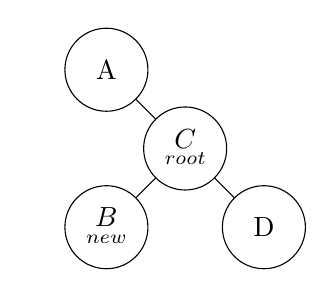
\begin{tikzpicture}[
            every node/.style = {minimum width = 3em, draw, circle},
            level/.style = {sibling distance = 20mm},
            level distance = 10mm
            ]
            \node{A}
            child {edge from parent[draw = none]}
            child {node {$\underset{root}{C}$}
                   child {node {$\underset{new}{B}$}}
                   child {node {D}}
                  };
          \end{tikzpicture}
      \vspace{4mm}
      \caption{The stick when a new node is inserted as a left child.}
    \end{subfigure}
    \hspace{1em}
    \begin{subfigure}[b]{0.3\linewidth}
        \centering
        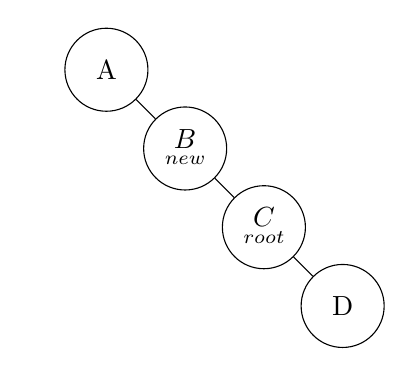
\begin{tikzpicture}[
            every node/.style = {minimum width = 3em, draw, circle},
            level/.style = {sibling distance = 20mm},
            level distance = 10mm
            ]
            \node{A}
            child {edge from parent[draw = none]}
            child {node {$\underset{new}{B}$}
                   child {edge from parent[draw = none]}
                   child {node {$\underset{root}{C}$}
                          child {edge from parent[draw = none]}
                          child {node {D}}
                         }
                  };
          \end{tikzpicture}
      \vspace{4mm}
      \caption{The reformed stick after \textsc{Stickify} is used on the tree from fig \ref{fig:stickify}a.}
    \end{subfigure}
    \hspace{1em}
    \begin{subfigure}[b]{0.3\linewidth}
        \centering
        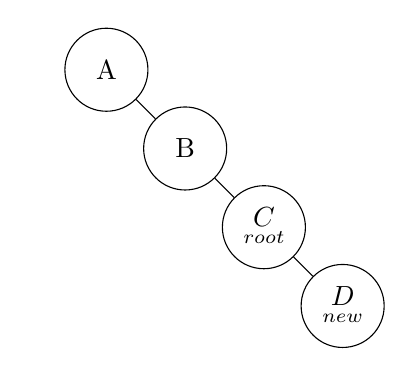
\begin{tikzpicture}[
            every node/.style = {minimum width = 3em, draw, circle},
            level/.style = {sibling distance = 20mm},
            level distance = 10mm
            ]
            \node{A}
            child {edge from parent[draw = none]}
            child {node {B}
                   child {edge from parent[draw = none]}
                   child {node {$\underset{root}{C}$}
                          child {edge from parent[draw = none]}
                          child {node {$\underset{new}{D}$}}
                         }
                  };
          \end{tikzpicture}
      \vspace{4mm}
      \caption{A case where $new.value$ is greater than $root.value$.}
    \end{subfigure}
    \caption{Examples of the 2 cases that \textsc{Stickify} has to deal with.}
    \label{fig:stickify}

\end{figure}

\end{document}